\section{Network synthesis for specified frequency dependent transfer functions} \label{network_synthesis}

In this section we describe how frequency dependent transfer functions represented as rational functions in tha laplace variable, s, may be simulated using passive circuits and hence modelled in Spice. We assume that the rational functions represent stable systems i.e. that their impulse response does not diverge as $t\rightarrow \inf$. This implies that the poles of the transfer function lie in the left hand side of the s plane.

We consider two types of transfer functions according to their properties
\begin{enumerate}
\item Positive-real transfer functions which may be represented as a one port network (simple impedance)
\item non-positive-real transfer functions which may be represented as two port networks
\end{enumerate}
%
The first type of transfer function arises in this work in the propagation correction functions. The second type may arise in transfer impedance models where the transfer resistance and/or inductance may be negative.

The form of the transfer functions that we wish to implement as a passive circuit are rational functions as in equation\ref{eq:rational_function}
%
\begin{equation} \label{eq:rational_function}
H\left(s\right)=\frac{a_{0}+a_{1}\left(\frac{s}{\omega_{0}}\right)+a_{2}\left(\frac{s}{\omega_{0}}\right)^{2}+\dots}{b_{0}+b_{1}\left(\frac{s}{\omega_{0}}\right)+b_{2}\left(\frac{s}{\omega_{0}}\right)^{2}+\dots}
\end{equation}
%
where $\omega_{0}$ is a frequency normalisation factor.
The methods applied make use of the work of Foster \cite{Foster}, Cauer\cite{Cauer} and Brune \cite{Brune}.

\subsection{One port impedance models}\label{one_port_imepdance_models}

A passive impedance function must be 'positive-real' to constitute a physical impedance which can be synthesised from a network of inductors, capacitors, resistors and transformers. A positive-real rational function is defined by the following conditions:

\begin{enumerate}
\item The real part of the function $Z(s)$ must be positive for all $s=\alpha+j\omega, \alpha>0$
\item The imaginary part of the function$Z(s)$ must be zero for all $s=\alpha+j\omega, \omega=0$
\end{enumerate}

Positive real rational functions have the following properties:

\begin{enumerate}
\item The number of poles and zeros differ by at most 1
\item The coefficients of the rational function are all real and positive
\item The poles and zeros of the function must lie in the left hand side of the s-plane or on the $s-j\omega$ axis
\item If a function $Z(s)$ is positive-real then so is $Y(s)=\frac{1}{Z(s)}$
\end{enumerate}

In this section we describe how an impedance represented as a rational function in s may be synthesised by a passive one port circuit consisting of resistors, inductors, capacitors and transformers i.e. spice R, L, C and K elements.
%
\begin{figure}[ht]
\centering
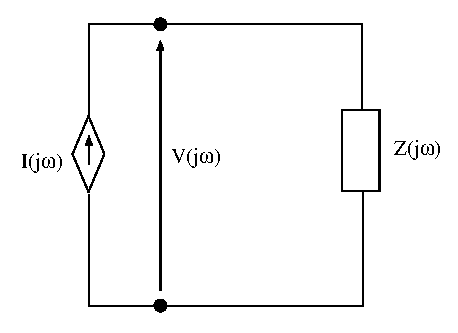
\includegraphics[scale=0.7]{./Imgs/one_port_network.eps}
\caption{One port network model of a positive-real transfer function}
\label{fig:one_port_network}
\end{figure}

Figure \ref{fig:one_port_network} shows a one port network driven by a current source $I\left\{ j \omega \right\}$ whose port voltage is given by $V\left\{ j \omega \right\}=Z\left\{ j \omega \right\}I\left\{ j \omega \right\}$. The impedance can be synthesised as a ladder network as shown in figure \ref{cauer_1}
%
\begin{figure}[ht]
\centering
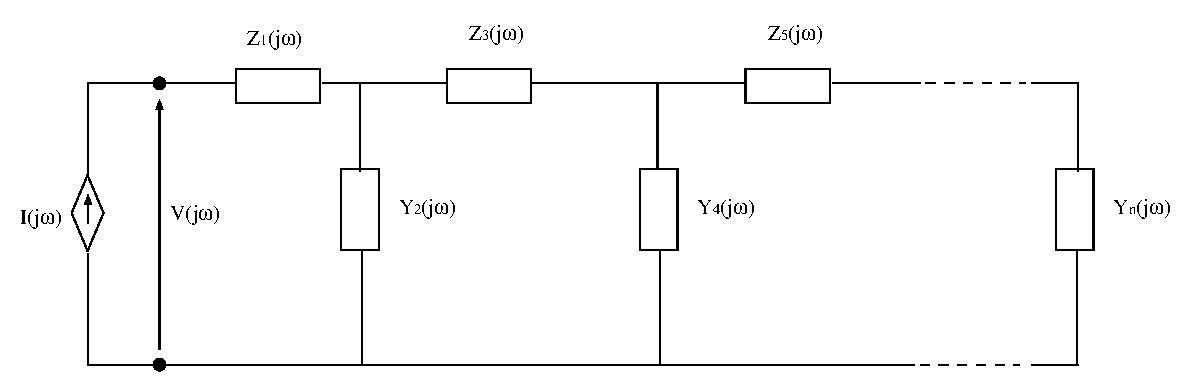
\includegraphics[scale=0.7]{./Imgs/cauer_1.eps}
\caption{Ladder network synthesis of an impedance}
\label{cauer_1}
\end{figure}
%
The impedance of the ladder network may be expressed as the sum of the first series impedance, $Z_1(s)$ and a remainder, $Z_{r1}(s)$ i.e.
%
\begin{equation} \label{eq:cauer_2}
Z\left(s\right)=Z_1(s)+Z_{r1}(s)
\end{equation}
%

The circuit is shown in figure \ref{cauer_2} where $Z_1(s)$ is the impedance of a combination of R, L, C, K elements and $Z_{r1}(s)$ is a stable positive real function.
%
\begin{figure}[ht]
\centering
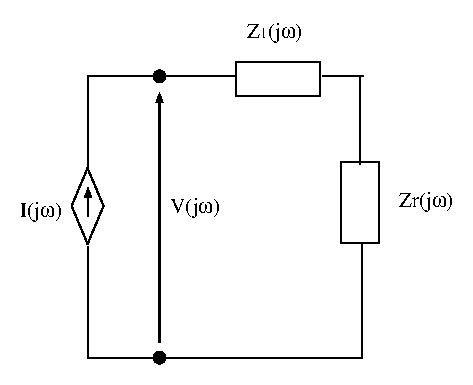
\includegraphics[scale=0.7]{./Imgs/cauer_2.eps}
\caption{Initial stage of ladder network synthesis}
\label{cauer_2}
\end{figure}
%
The remainder impedance, $Z_{r1}(s)$, is then synthesised as the parallel combination of the admittance function  $Y_2(s)$ and a remainder, $Y_{r2}(s)$ as seen in figure \ref{cauer_3}
%
\begin{equation} \label{eq:cauer_2a}
Z_{r1}(s)=\frac{1}{Y_2(s)+Y_{r2}(s)}
\end{equation}
%
thus
%
\begin{equation} \label{eq:cauer_2b}
Z\left(s\right)=Z_1(s)+\frac{1}{Y_2(s)+Y_{r2}(s)}
\end{equation}
%
The admittance $Y_{r2}(s)$ is then synthesised as the sum of two series impedances i.e. 
%
\begin{equation} \label{eq:cauer_2c}
Z\left(s\right)=Z_1(s)+\cfrac{1}{Y_2(s)+  \cfrac{1}{Z_3(s)+ Z_{r3}(s)  } }
\end{equation}
%
It is seen from this that the impedance function of the ladder network is expressed in a continued fraction form with alternating impedance and admittance terms. 
This synthesis procedure in which admittance and impedance elements of the ladder network are identified in turn continues until the remainder term is reduced to zero. This leads to a relatively straightforward synthesis process for impedance functions.

\begin{figure}[ht]
\centering
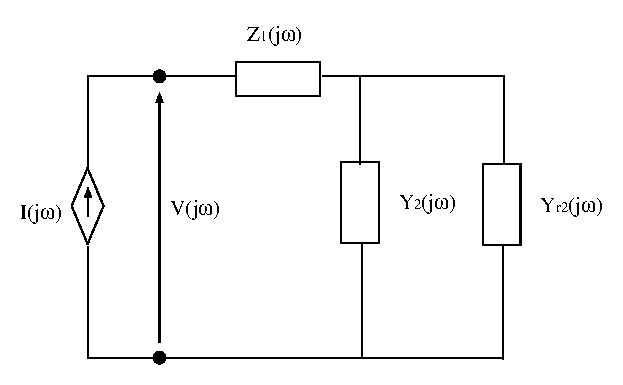
\includegraphics[scale=0.7]{./Imgs/cauer_3.eps}
\caption{Second stage of ladder network synthesis}
\label{cauer_3}
\end{figure}
%

\subsection{Algorithm for impedance synthesis} 

The starting point for the algorithm for impedance synthesis is a rational function in s which must be stable and positive-real. The impedance is synthesised by extracting series impedances and parallel admittances in turn until the remainder is zero. The impedance/ admittance extraction makes use of a pole-residue representation of the transfer function in order to identify branches which are combinations of R, L and C elements. This method can get stuck in that a viable branch cannot be identified while leaving a stable positive-real remainder function. In this case a technique developed by Brune \cite{Brune} is used to continue the synthesis. Brune's method makes use of transformers (K elements in Spice).  

An outline of the algorithm is as follows:

\begin{enumerate}
\item Attempt to identifiy a viable series impedance branch i.e. a branch which may be synthesised with R, L, and C elements and which leaves a remainder $Z_r(s)$ which is stable and posistive-real. If a viable branch is found then this process can be repeated until no further viable series impedance brances can be found.
\item Once no futher viable series impedance contributions can be found, calculate the admittance $Y_r(s)=1/Y_r(s)$ and attempt to identifiy a viable parallel admittance branch i.e. a branch which may be synthesised with R, L, and C K elements and which leaves a remainder $Y_r(s)$ which is stable and posistive-real. If a viable branch is found then this process can be repeated until no further viable parallel admittance brances can be found.
\item If no viable series impedance branches or parallel admittance branches can be found then use the Brune synthesis method and implement the resulting circuit with R, L, C and K elements
\item Return to step 1 and repeat until the remainder impedance/ admittance is zero.
\end{enumerate}

\subsection{Identification of series impedance branches} 
A vaiable series impedance branch can be one of the following:

\begin{enumerate}
\item  RLC in parallel branch
\item  LC in parallel branch
\item  RC in parallel branch
\item  RL in parallel branch
\item  C branch
\item  L branch
\item  R branch (which may be identified in two different ways)
\end{enumerate}

These branches are shown in figure \ref{fig:series_impedance_branches}

\begin{figure}[ht]
\centering
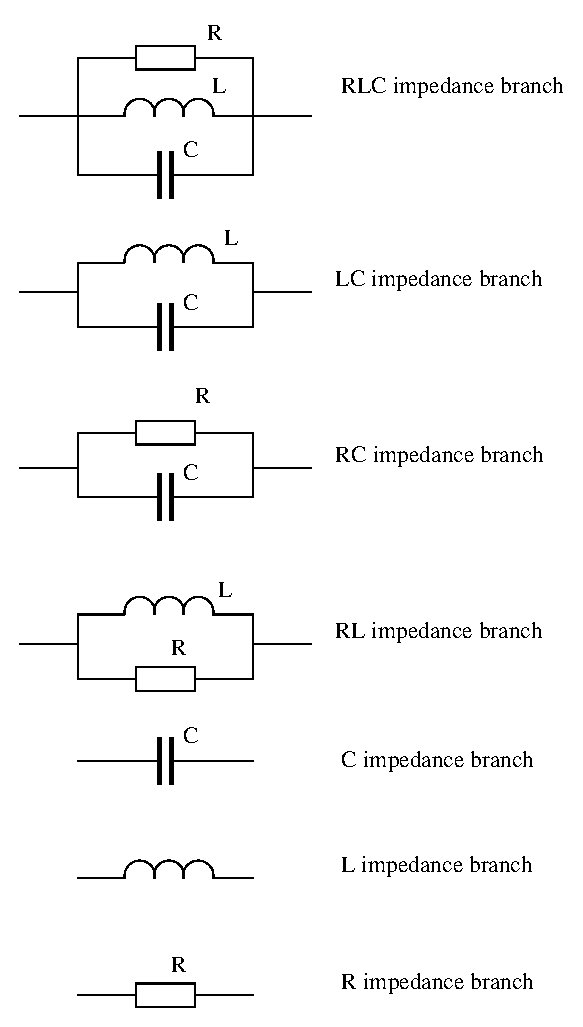
\includegraphics[scale=0.7]{./Imgs/series_impedance_branches.eps}
\caption{Series Impedance Branches}
\label{fig:series_impedance_branches}
\end{figure}
%
Viable branches are found by first forming a pole-residue expansion of the impedance function where poles and their corresponding residues may be real or may be complex conjugate pairs i.e. 
%
\begin{equation} \label{eq:rational_function_Z}
Z\left(s\right)=R+sL+\sum_{i=1}^{n\_real\_poles} \frac{r_i}{s-p_i} + 
                           \sum_{i=1}^{n\_complex\_pole\_pairs} \frac{r_i}{s-p_i}+\frac{r_i^*}{s-p_i^*}
\end{equation}
%
Then each of the branch types is looked for in the pole-residue expansion in the order of the above list. Each of the following subsections shows how each of the above branch types may be identified from the pole-residue expansion.

\subsubsection{RLC in parallel branch}

The RLC parallel branch has an impedance function which can be expressed in rational function as
\begin{equation} 
Z\left(s\right)=\frac{\frac{s}{C}}{\frac{1}{L C} + \frac{s}{C R} + s^2}
\end{equation}
This may be expressed in pole-residue form as the complex pole-residue pair
\begin{equation} 
Z\left(s\right)= \frac{r}{s-p}+\frac{r^*}{s-p^*}=\frac{\left(rp^*-r^*p\right)+\left( r+r^*\right)s}{pp^*-\left( p+p^*\right)s+s^2}
\end{equation}
Where the poles are complex (and not purely imaginary). Equating coefficients of the rational functions a requirement for a viable RLC parallel branch can be established i.e. the numerator constant term is zero:
\begin{equation} 
rp^*-r^*p=0
\end{equation}
In addition we require that all the component values of the parallel RLC circuit be positive i.e.
\begin{equation} 
C=\frac{1}{r+r^*}>0
\end{equation}
\begin{equation} 
L=\frac{r+r^*}{pp^*}>0
\end{equation}
\begin{equation} 
R=\frac{r+r^*}{p+p^*}>0
\end{equation}
The final requirement is that the remainder function be positive real i.e. the remaining terms of the impedance function describe a physical impedance. If these requirements are satisfied then a parallel RLC branch can be extracted from the impedance function and implemented as a series impedance branch in the ladder network. 

\subsubsection{LC in parallel branch}

The LC parallel branch has an impedance function which can be expressed in rational function as
\begin{equation} 
Z\left(s\right)=\frac{\frac{s}{C}}{\frac{1}{L C} + s^2}
\end{equation}
This is a special case of the RLC branch in which $R\rightarrow \inf$ may be expressed in pole-residue form as the complex pole-residue pair
\begin{equation} 
Z\left(s\right)= \frac{r}{s-p}+\frac{r^*}{s-p^*}=\frac{\left(rp^*-r^*p\right)+\left( r+r^*\right)s}{pp^*-\left( p+p^*\right)s+s^2}
\end{equation}
Where the poles are purely imaginary. Equating coefficients of the rational functions a requirement for a viable LC parallel branch can be established i.e. the poles are imaginary:
\begin{equation} 
p^*+p=0
\end{equation}
The numerator constant term is zero:
\begin{equation} 
rp^*-r^*p=0
\end{equation}
In addition we require that all the component values of the parallel LC circuit be positive i.e.
\begin{equation} 
C=\frac{1}{r+r^*}>0
\end{equation}
\begin{equation} 
L=\frac{r+r^*}{pp^*}>0
\end{equation}
The final requirement is that the remainder function be positive real i.e. the remaining terms of the impedance function describe a physical impedance. If these requirements are satisfied then a parallel RLC branch can be extracted from the impedance function and implemented as a series impedance branch in the ladder network. 

\subsubsection{RC in parallel branch}

The RC parallel branch has an impedance function which can be expressed in rational function as
\begin{equation} 
Z\left(s\right)=\frac{\frac{1}{C}}{\frac{1}{R C} + s}
\end{equation}
This may be expressed in pole-residue form as
\begin{equation} 
Z\left(s\right)= \frac{r}{s-p}
\end{equation}
Where the pole and residue are both real. By equating coefficients of the functions, values of R and C can be identified
We require that all the component values of the parallel RC circuit be positive i.e.
\begin{equation} 
C=\frac{1}{r}>0
\end{equation}
\begin{equation} 
R=\frac{-r}{p}>0
\end{equation}
The final requirement is that the remainder function be positive real i.e. the remaining terms of the impedance function describe a physical impedance. If these requirements are satisfied then a parallel RC branch can be extracted from the impedance function and implemented as a series impedance branch in the ladder network. 


\subsubsection{RL in parallel branch}

The RL parallel branch has an impedance function which can be expressed in rational function as
\begin{equation} 
Z\left(s\right)=\frac{sR}{\frac{R}{L} + s}=R-\frac{\frac{R^2}{L}}{s+\frac{R}{L}}
\end{equation}
As for the parallel RC branch, this may be expressed in pole-residue form, including a constant term as
\begin{equation} 
Z\left(s\right)= K+\frac{r}{s-p}
\end{equation}
Where the pole and residue are both real. By equating coefficients of the functions, values of R and L can be identified
We require that all the component values of the parallel RL circuit be positive i.e.
\begin{equation} 
R=\frac{r}{p}>0
\end{equation}
\begin{equation} 
L=\frac{-r}{p^2}>0
\end{equation}
The final requirement is that the remainder function be positive real i.e. the remaining terms of the impedance function describe a physical impedance. If these requirements are satisfied then a parallel RC branch can be extracted from the impedance function and implemented as a series impedance branch in the ladder network. 


\subsubsection{Capacitance branch}

The capacitance branch has an impedance function which consists of a pole at zero i.e.
\begin{equation} 
Z\left(s\right)=\frac{1}{sC}
\end{equation}
Thus in the pole-residue expansion we require a pole at zero. In addition we require that capacitance be positive i.e.
\begin{equation} 
C=\frac{1}{r}>0
\end{equation}
The final requirement is that the remainder function be positive real i.e. the remaining terms of the impedance function describe a physical impedance. If these requirements are satisfied then a capacitance branch can be extracted from the impedance function and implemented as a series impedance in the ladder network. 


\subsubsection{Inductance branch}

The inductance branch has an impedance given by
\begin{equation} 
Z\left(s\right)=sL
\end{equation}
Thus in the pole-residue expansion we require a $sL$ term (pole at infinity in the impedance function) with positive inductance, L.
The final requirement is that the remainder function be positive real i.e. the remaining terms of the impedance function describe a physical impedance. If these requirements are satisfied then an inductance branch can be extracted from the impedance function and implemented as a series impedance in the ladder network. 

\subsubsection{Resistance branch, type 1}

The resistance branch of type 1 is identified by a positive constant term in the pole-residue expansion of the impedance. If the remainder function is positive real i.e. the remaining terms of the impedance function describe a physical impedance then a resistance branch can be extracted from the impedance function and implemented as a series impedance in the ladder network. 

\subsubsection{Resistance branch, type 2}

The resistance branch of type 2 may be found from the rational function form of the impedance i.e. if
%
\begin{equation} \label{eq:rational_function_R2}
Z\left(s\right)=\frac{a_{0}+a_{1}\left(\frac{s}{\omega_{0}}\right)+a_{2}\left(\frac{s}{\omega_{0}}\right)^{2}+\dots}{b_{0}+b_{1}\left(\frac{s}{\omega_{0}}\right)+b_{2}\left(\frac{s}{\omega_{0}}\right)^{2}+\dots}
\end{equation}
%
then we can calculate the resistance, $R$ as
%
\begin{equation} \label{eq:rational_function_R2b}
R=\frac{a_{0}}{b_{0}}
\end{equation}
%
as opposed to the pole-residue form whose constant (resistance) term is found as the ratio of the numerator and denominator coefficients of the highest power of s 
%
subtracting the resistance as defined in \ref{eq:rational_function_R2b} results in a remainder inmpedance function with a pole at infinity. As for all the othetr branch identification methods, this resistance branch can only be extracted if the remainder impedance is a stable physical impedance function. 


%_______________________________________________________________________________________________
%


\subsection{Identification of admittance branches} 

A vaiable admittance branch can be one of the following:

\begin{enumerate}
\item  RLC in series branch
\item  LC in series branch
\item  RC in series branch
\item  RL in series branch
\item  C branch
\item  L branch
\item  R branch (which may be identified in two different ways)
\end{enumerate}

These branches are shown in figure \ref{fig:parallel_admittance_branches} and are seen to be the duals of the corresponding impedance branches in figure \ref{fig:series_impedance_branches}. The dual circuits are found by the transformations

\begin{equation} \label{eq:dual_circuits}
\begin{array}{rcl}
Z & \leftrightarrow & Y \\
L & \leftrightarrow & C \\
\frac{1}{C} & \leftrightarrow & \frac{1}{L} \\
R & \leftrightarrow & G
\end{array}
\end{equation}

\begin{figure}[ht]
\centering
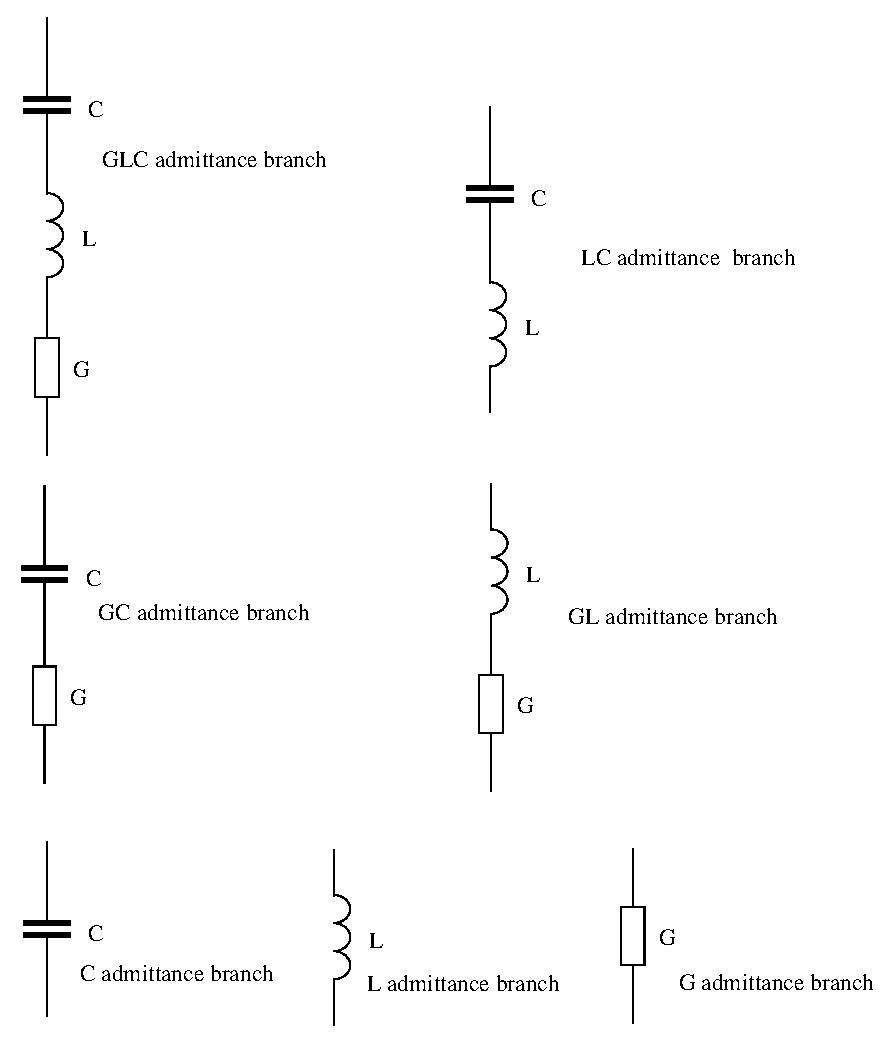
\includegraphics[scale=0.7]{./Imgs/parallel_admittance_branches.eps}
\caption{Parallel Admittance Branches}
\label{fig:parallel_admittance_branches}
\end{figure}
%
The admittance branches are found in the same was as for the series impedance branches i.e. viable branches are found by first forming a pole-residue expansion of the admittance function where poles and their corresponding residues may be real or may be complex conjugate pairs i.e. 
%
\begin{equation} \label{eq:rational_function_Y}
Y\left(s\right)=G+sC+\sum_{i=1}^{n\_real\_poles} \frac{r_i}{s-p_i} + 
                           \sum_{i=1}^{n_complex\_pole\_pairs} \frac{r_i}{s-p_i}+\frac{r_i^*}{s-p_i^*}
\end{equation}
%
For completeness a brief summary of the admittance branch identification processes is given here. The admittances may have inductance, capacitance or conductance though a non-zero conductance is implemented as a resistance $R=/frac{1}{G}$ in Spice.

\subsubsection{GCL in series branch}

The GCL series branch has an admittance function which can be expressed in rational function as
\begin{equation} 
Y\left(s\right)=\frac{\frac{s}{L}}{\frac{1}{C L} + \frac{s}{L G} + s^2}
\end{equation}
This may be expressed in pole-residue form as the complex pole-residue pair
\begin{equation} 
Y\left(s\right)= \frac{r}{s-p}+\frac{r^*}{s-p^*}=\frac{\left(rp^*-r^*p\right)+\left( r+r^*\right)s}{pp^*-\left( p+p^*\right)s+s^2}
\end{equation}
The poles are complex (and not purely imaginary). Equating coefficients of the rational functions a requirement for a viable GCL series branch can be established i.e. the numerator constant term is zero:
\begin{equation} 
rp^*-r^*p=0
\end{equation}
In addition we require that all the component values of the series GCL circuit be positive i.e.
\begin{equation} 
L=\frac{1}{r+r^*}>0
\end{equation}
\begin{equation} 
C=\frac{r+r^*}{pp^*}>0
\end{equation}
\begin{equation} 
G=\frac{r+r^*}{p+p^*}>0
\end{equation}
The final requirement is that the remainder function be positive real i.e. the remaining terms of the admittance function describe a physical admittance. If these requirements are satisfied then a series GCL branch can be extracted from the admittance function and implemented as a parallel admittance branch in the ladder network. 

\subsubsection{LC in series branch}

The LC series branch has an admittance function which can be expressed in rational function as
\begin{equation} 
Y\left(s\right)=\frac{\frac{s}{L}}{\frac{1}{C L} + s^2}
\end{equation}
This is a special case of the GCL branch in which $G \rightarrow \inf$ ($R \rightarrow 0$) may be expressed in pole-residue form as the complex pole-residue pair
\begin{equation} 
Y\left(s\right)= \frac{r}{s-p}+\frac{r^*}{s-p^*}=\frac{\left(rp^*-r^*p\right)+\left( r+r^*\right)s}{pp^*-\left( p+p^*\right)s+s^2}
\end{equation}
Where the poles are purely imaginary. Equating coefficients of the rational functions a requirement for a viable LC series branch can be established i.e. the poles are imaginary:
\begin{equation} 
p^*+p=0
\end{equation}
The numerator constant term is zero:
\begin{equation} 
rp^*-r^*p=0
\end{equation}
In addition we require that all the component values of the series LC circuit be positive i.e.
\begin{equation} 
L=\frac{1}{r+r^*}>0
\end{equation}
\begin{equation} 
C=\frac{r+r^*}{pp^*}>0
\end{equation}
The final requirement is that the remainder function be positive real i.e. the remaining terms of the admittance function describe a physical admittance. If these requirements are satisfied then a series GCL branch can be extracted from the admittance function and implemented as a parallel admittance branch in the ladder network. 

\subsubsection{GL in series branch}

The GL series branch has an admittance function which can be expressed in rational function as
\begin{equation} 
Y\left(s\right)=\frac{\frac{1}{L}}{\frac{1}{G L} + s}
\end{equation}
This may be expressed in pole-residue form as
\begin{equation} 
Y\left(s\right)= \frac{r}{s-p}
\end{equation}
Where the pole and residue are both real. By equating coefficients of the functions, values of G and L can be identified
We require that the component values of the series GL circuit be positive i.e.
\begin{equation} 
L=\frac{1}{r}>0
\end{equation}
\begin{equation} 
G=\frac{-r}{p}>0
\end{equation}
The final requirement is that the remainder function be positive real i.e. the remaining terms of the admittance function describe a physical admittance. If these requirements are satisfied then a series GL branch can be extracted from the admittance function and implemented as a parallel admittance branch in the ladder network. 


\subsubsection{GC in series branch}

The GC series branch has an admittance function which can be expressed in rational function as
\begin{equation} 
Y\left(s\right)=\frac{sG}{\frac{G}{C} + s}=G-\frac{\frac{G^2}{C}}{s+\frac{G}{C}}
\end{equation}
As for the series GL branch, this may be expressed in pole-residue form, including a constant term as
\begin{equation} 
Y\left(s\right)= K+\frac{r}{s-p}
\end{equation}
Where the pole and residue are both real. By equating coefficients of the functions, values of G and C can be identified
We require that all the component values of the series GC circuit be positive i.e.
\begin{equation} 
G=\frac{r}{p}>0
\end{equation}
\begin{equation} 
C=\frac{-r}{p^2}>0
\end{equation}
The final requirement is that the remainder function be positive real i.e. the remaining terms of the admittance function describe a physical admittance. If these requirements are satisfied then a series GL branch can be extracted from the admittance function and implemented as a parallel admittance branch in the ladder network. 


\subsubsection{Inductance branch}

The inductance branch has an admittance function which consists of a pole at zero i.e.
\begin{equation} 
Y\left(s\right)=\frac{1}{sL}
\end{equation}
Thus in the pole-residue expansion we require a pole at zero. In addition we require that inductance be positive i.e.
\begin{equation} 
L=\frac{1}{r}>0
\end{equation}
The final requirement is that the remainder function be positive real i.e. the remaining terms of the admittance function describe a physical admittance. If these requirements are satisfied then a inductance branch can be extracted from the admittance function and implemented as a parallel admittance in the ladder network. 


\subsubsection{Capacitance branch}

The capacitance branch has an admittance given by
\begin{equation} 
Y\left(s\right)=sC
\end{equation}
Thus in the pole-residue expansion we require a $sC$ term (pole at infinity in the admittance function) with positive capacitance, C.
The final requirement is that the remainder function be positive real i.e. the remaining terms of the admittance function describe a physical admittance. If these requirements are satisfied then an capacitance branch can be extracted from the admittance function and implemented as a parallel admittance in the ladder network. 

\subsubsection{Conductance (Resistance) branch, type 1}

The resistance branch of type 1 is identified by a positive constant term in the pole-residue expansion of the admittance. If the remainder function is positive real i.e. the remaining terms of the admittance function describe a physical admittance then a resistance branch can be extracted from the admittance function and implemented as a parallel admittance in the ladder network. 

\subsubsection{Conductance (Resistance) branch, type 2}

The resistance branch of type 2 may be found from the rational function form of the admittance i.e. if
%
\begin{equation} \label{eq:rational_function_G2}
Y\left(s\right)=\frac{a_{0}+a_{1}\left(\frac{s}{\omega_{0}}\right)+a_{2}\left(\frac{s}{\omega_{0}}\right)^{2}+\dots}{b_{0}+b_{1}\left(\frac{s}{\omega_{0}}\right)+b_{2}\left(\frac{s}{\omega_{0}}\right)^{2}+\dots}
\end{equation}
%
then we can calculate the conductance, $G$ as
%
\begin{equation} \label{eq:rational_function_G2b}
G=\frac{a_{0}}{b_{0}}
\end{equation}
%


\clearpage

%_______________________________________________________________________________________________
%
\subsection{Brune Synthesis} 

There are circumstances when the ladder network synthesis procedure described above fails i.e. a physical impedance/ admittance function results for which no viable series impedance or parallel admittance branch can be found. In this case the method described by Brune \cite{Brune} may be applied to allow the process to proceeed. Brune's method involves the use of a transformer which can be included in Spice simulations using the K element. The basic process is described here however the associated proofs of the properties of the functions at each stage will not be given. For further details see reference \cite{Brune}.

The ladder network synthesis procedure ensures that poles at zero, poles at infinity, zeros at infinity, zeros at zero, poles on the $s=\pm j\omega$ axis and zeros on the $s=\pm j\omega$ axis have been removed from the impedance function. Brune's method then operates on this remainer function, $Z_r(s)$, as follows:

Stage 1. Find $\omega_0$ such that the real part of the impedance $Z_r(s=j\omega_0)$ is a minimum. The minimum resistance value a this frequency is $R_{min}$.

Stage 2. Subtract $R_{min}$ from $Z_r(s)$ to give the minimum resistance impedance function 

\begin{equation} \label{eq:brune_1}
Z_1\left(s\right)=Z_r\left(s\right)-R_{min}
\end{equation}
i.e. $R_{min}$ is extracted as a series resistance.

The function $Z_1\left(s\right)$ is now purely reactive at $w_0$ i.e. $Z_1\left(\omega_0\right)=jX$. This reactance is set to be the reactance of an inductor, $L_A$ where $L_A=\frac{X}{\omega_0}$. Note that this inducatance may be negative. 

This series inductance is subtracted from $Z_1(s)$ to give

\begin{equation} \label{eq:brune_2}
Z_2\left(s\right)=Z_1\left(s\right)-sL_A
\end{equation}

$Z_2\left(s\right)$ has a zero of order 2 at $s=j\omega_0$ and we can write the admittance $Y_2(s)=\frac{1}{Z_2(s)}$ as

\begin{equation} \label{eq:brune_3}
Y_2\left(s\right)=\frac{1}{Z_1\left(s\right)-sL_A}=\frac{\alpha}{s^2+\omega_0^2}+Y_3\left(s\right)
\end{equation}

From this we can identify a LC admittance branch where $L_B=\frac{1}{\alpha}$ and $C_B=\frac{1}{\omega_0^2 L_B}$

The remainder impedance $Z_3\left(s\right)=\frac{1}{Y_3\left(s\right)}$ after subtraction of the LC admittance branch has a first order pole at infinity and therefore a series inductance can be extracted i.e. 

\begin{equation} \label{eq:brune_4}
Z_r\left(s\right)=Z_3\left(s\right)-sL_C
\end{equation}

where $L_C$ is negative if $L_A$ is positive and vice versa. In addition to this it can be shown that the remainder impedance, $Z_r(s)$ is positive-real.

This series of component identification leads to the circuit shown in figure \ref{fig:Brune_1} however this is not a physical circuit in that one of the series inductors $L_A$ or $L_B$ is negative. The three inductances may be combined into two positive inductors with a mutual inductance term as seen in figure \ref{fig:Brune_2}. In this circuit the component values can be shown to be

\begin{equation} \label{eq:brune_5}
\begin{array}{rcl}
L_1 & = & L_A+L_0 \\
L_2 & = & L_B+L_0\\
K & = & 1\\
\end{array}
\end{equation}

The inductances in the final Brune synthesis circuit are all positive and may therefore be simulated in Spice using L, C R and K elements. Since the remainder impedance is positive-real, the ladder network synthesis procedure can proceed.

\begin{figure}[ht]
\centering
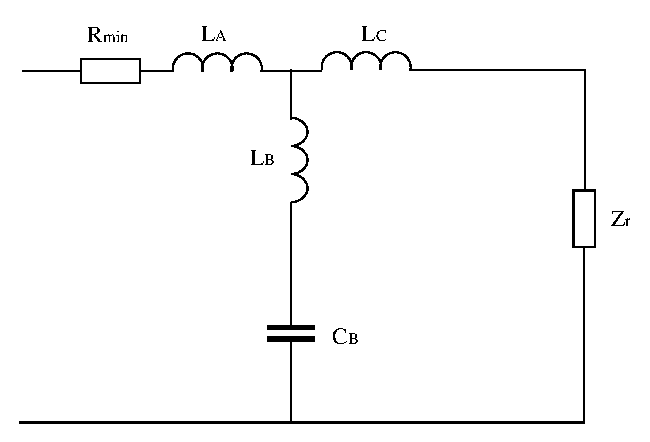
\includegraphics[scale=0.7]{./Imgs/Brune_1.eps}
\caption{Initial Brune Synthesis Circuit}
\label{fig:Brune_1}
\end{figure}
%

\begin{figure}[ht]
\centering
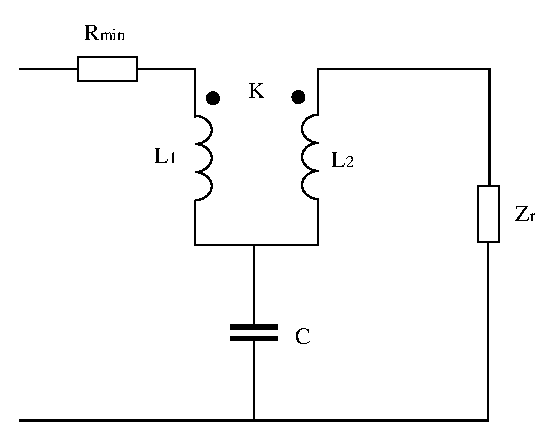
\includegraphics[scale=0.7]{./Imgs/Brune_2.eps}
\caption{Final Brune Synthesis Circuit}
\label{fig:Brune_2}
\end{figure}
%

